\documentclass[a4paper]{article}

\usepackage[english]{babel}
\usepackage[utf8]{inputenc}
\usepackage{amsmath}
\usepackage{graphicx}
\usepackage[colorinlistoftodos]{todonotes}

\title{Entertainment Rating Based on Twitter
Sentiment Analysis}

\author{Gauri Sunil Kolhe - 409023002, Pratheek Basavana Gowda - 993957668,\\ Pavan
Nagathihalli Shankarappa - 398768354}

\date{\today}

\begin{document}
\maketitle

\begin{abstract}
With microblogging platforms such as Twitter generating
huge amounts  of textual data every day, the possibilities of knowledge
discovery through Twitter data becomes increasingly relevant. Similar
to the public voting mechanism on websites such as the Internet Movie
Database (IMDb) that aggregates movies ratings, Twitter content contains
reflections of public opinion about movies. This study aims to explore
the use of Twitter content as textual data for predicting the entertainment
rating. In this study, we will be extracting tweets from the
Twitter API and predict the sentiment involved.Each tweet that we extract
from the twitter should be categorized as a positive or negative
tweet. We calculate the rating by the total of positive tweets by the total
number of tweets.Results will be showing rating developed by our
application is compared to IMDB and Rotten Tomatoes.
\end{abstract}

\section{INTRODUCTION}
\label{sec:introduction}

The movie rating prediction by extracting the tweets and hashtags related to a specific movie. Twitter data can be accessed through the public API provided by the Twitter. The authentication request grant the access to these APIs, which must be signed with valid login and password. Twitter provides authentication keys for extractions of the tweets.
Tweet extracted from twitter API is collected in MySql where the tweet is having a unique tweet id, tweet movie name and tweet description. Movie name is added by user as an input and we are extracting tweet Id of the movie from the twitter and all the tweets are extracted from the twitter. We have update the tweets of the movie by establishing the connection with twitter from our application and then recent 1000 tweets are stored in our database. We have also calculated the popularity of the movie at the time we extract tweets. Each time we want to predict the rating or calculate the popularity of movie labelling of every tweet is also calculated. Apart from the tweets obtained from Twitter, the application also calculates the sentiment associated with the tweet. The application also stores the sentiment associated with the tweet in the database. Sentiment of a tweet is categorized as positive, negative and neutral. In this application we trained a classifier to classify tweets in positive, negative and neutral. This is the backbone of our application. Each tweet that we extract from the twitter should be categorized as positive or negative tweet. For calculating the movie rating we ignored neutral tweets as these are not useful for any type of information for movie review. For movie rating prediction we have designed a module by which you can select any movie and all the tweets related to that movie is loaded in the algorithm with hashtags of the movie is also added so that all the review is added for the particular movie and more precise and accurate rating is calculated by using two different techniques as NLTK and TextBlob. When we search for a movie which is twitter id of the movie then rating out of 10 is calculated.
The performance of this application is evaluated by comparing its results with results from popular movie rating websites like IMDB and Rotten Tomatoes. The rating calculated for various movies released by fetching tweets related to the movie is stored in our application and real time rating of the movie is calculated and is represented in tabular form and graphically. The ratings collected show that the Twitter rating application is following similar trends as shown in IMDB and Rotten Tomatoes. Ratings from Twitter application are observed to be of a lower value. This can be attributed to the fact that the number of users rating a movie on the other websites is almost 100x times than what the Twitter application is using. A small experiment was conducted with varying number of tweets used by Twitter application to confirm this theory.

\section{RELATED WORK}
\label{sec:relatedwork}
The topic of using social media to predict the future becomes
very popular in recent years. Different work has been already
done using twitter content for predicting the sentiment of
tweets. Movie sentiment analysis based on public tweets \cite{ref1}
,In this paper they introduced a special approach to
understanding the tongue and frequency of words from one 
sentiment category enabling a much better sentiment
classification compared to the normal machine learning
techniques. They additionally introduce an added sentiment
category - the neutral category. In their analysis they use the
Python programming language with the NLTK library and
compare so obtained results with the normal machine
learning. Predicting Ratings for New Movie Releases from
Twitter Content that is textual knowledge from Twitter
will be seen as an in depth supply of data relating to a
particularly broad form of subjects. With a lot of users
actively expressing themselves on-line, a large quantity of
information is generated daily. Since this knowledge for an
over sized half consists of human expressions, Twitter
knowledge will be seen as a valuable assortment of human
opinion or sentiment, which might be mechanically extracted
with comparatively high accuracy.

\section{METHODOLOGY}
The overall system can be designed in following phases
\begin{itemize}
  \item Tweet Collection.
  \item Tweet Classification.
  \item Algorithm for Tweet Classification.
  \item Rating Movies.
\end{itemize}


\subsection{Tweet Collection}
Twitter data can be accessed through the public API provided
by the Twitter. These APIs can be accessed only by
authentication requests, which must be signed with valid login
ID and password. Twitter provides authentication keys for
extractions of the tweets.We have the following unique keys that is
required to fetch tweets from twitter
\begin{itemize}
\item Consumer key
\item Consumer Secret key
\item Access token
\item Access token secret
\end{itemize}
Tweet Extracted from twitter having complete information
like date of tweet, tweet ID, user ID, retweet count etc.We
will use only tweet ID and tweet description. We have integrated
twitter API into our application so as to fetch all the tweets
related to a particular movie.The tweets are
collected into the MySQL database. We have to update the tweets of the movie by
establishing the connection with twitter from our application,
and then all the recent tweets are added to our database.

\subsection{Tweet Classification}
In this module I label every tweet as positive, negative and
neutral.Each time we want to predict the rating
or calculate the popularity of movie and labeling of every
tweet is also calculated. Apart from the tweets obtained from 
Twitter, the application also calculates the sentiment
associated with the tweet. In this we pass the tweet through two sentiment analyzers TextBlob and NLTK classifiers which calculate the polarity and subjectivity of the tweets. The tweets are then labeled as positive, negative and neutral. We calculate the rating based on the positive  and negative tweets ignoring neutral tweets.  
\subsubsection{NLTK}
We have achieved a voting system to choose the best out of all the learning methods that has been trained in the NLP module of the project using NLTK 3 and sklearn. The Models that are trained Using sklearn are 
\begin{itemize}
\item  Naive Bayes:
\begin{itemize}
\item MultinomialNB
\item BernoulliNB
\end{itemize} 
\item Linear Model
\begin{itemize}
\item LogisticRegression:
\item  SGDClassifier:
\end{itemize} 
\item SVM
\begin{itemize}
\item  SVC
\item LinearSVC
\item NuSVC
\end{itemize}
\end{itemize}
We get the polarity of the tweet that we pass to this module and the confidence measure of the classifier about the polarity that is decided. 

\subsubsection{TextBlob}
TextBlob is a Python (2 and 3) library for processing textual data. It provides a simple API for diving into common natural language processing (NLP) tasks such as part-of-speech tagging, noun phrase extraction, sentiment analysis, classification, translation, and more. 
The sentiment property returns a namedtuple of the form Sentiment(polarity, subjectivity). The polarity score is a float within the range [-1.0,1.0]. The subjectivity is a float within the range [0.0, 1.0] where 0.0 is very objective and 1.0 is very subjejctive.
\subsection{Algorithm for Tweet Classification}
\begin{enumerate}
\item  Extract the tweet from twitter using Twitter API.
\item  Store the tweet in the database. Each tweet has a unique id
and tweet description with movie name which is also store in the database.
\item  For each tweet we have to specify the tweet label. Tweet
labels are positive, negative.
\item Calculate the value of p and n i.e. total number of positive
and negative tweets obtained by doing NLP on the machine. 
\item  Classify the tweet label of each tweet using the following
formula
\end{enumerate}
\begin{itemize}
\item For NLTK analysis if the confidence rating is above 0.5 only then we consider them as a valid polarity measure and label that tweet as positive or negative.
\item For Text blob analysis if the polarity is above 0 we consider that as a positive tweet and if polarity is less then 0 the tweet is consider as negative.
\end{itemize}
\subsection{Rating Movie}
\[rating = \frac{Positive Tweets}{Positive Tweets + Negative Tweets}  *  10\]
Rating is taken in the scale of 1 - 10.
Positive Tweet = Total number of tweets with positive label.
Negative Tweet = Total number of tweets with negative label.
The rating is multiplied with 10 to normalize it to the scale of 10. 
\section{SCREENSHOT OF APPLICATION}
Screenshot 1 = Without any inputs given.
\section{EXPERIMENTAL RESULTS AND
PERFORMANCE ANALYSIS}
The performance of this application is evaluated by comparing its results with results from popular movie rating websites like IMDB and Rotten Tomatoes. IMDB is internet information of data associated with films, television, programs etc. the location permits registered users to rate any film on a scale of one to ten, except for writing reviews regarding it. The location displays a weighted mean of user ratings and displays it next to the movie title. 
This website has 6.05 Daily Page views per visitor and a median of fifteen million individuals visit the web site per month. Rotten Tomatoes may be a web site dedicated to film reviews and news. It offers 2 sorts of scores for movies – Tomato meter critic mixture score and Audience score. The Critic mixture score reflects reviews and ratings from varied newspaper writers or from those that belong to film critic associations. The Audience score is calculated supported user’s reviews and ratings. For the aim of confirmatory this application, solely Audience score is taken into account. Registration is free however the location requests permission to look at user’s social network profiles. It gets 3.60 Daily Page views per visitor and a median of thirteen million individuals visit the web site per month. The rating calculated for various movies released by fetching tweets related to the movie is stored in our application and real time rating of the movie is calculated and is represented in and graphically. Since rotten tomatoes has not yet provided us with the api access we where not able to integrate it with the application hence we have hard coded the values for such movies and can be integrated when the access is provided. 
\begin{figure}[h!]
\centering
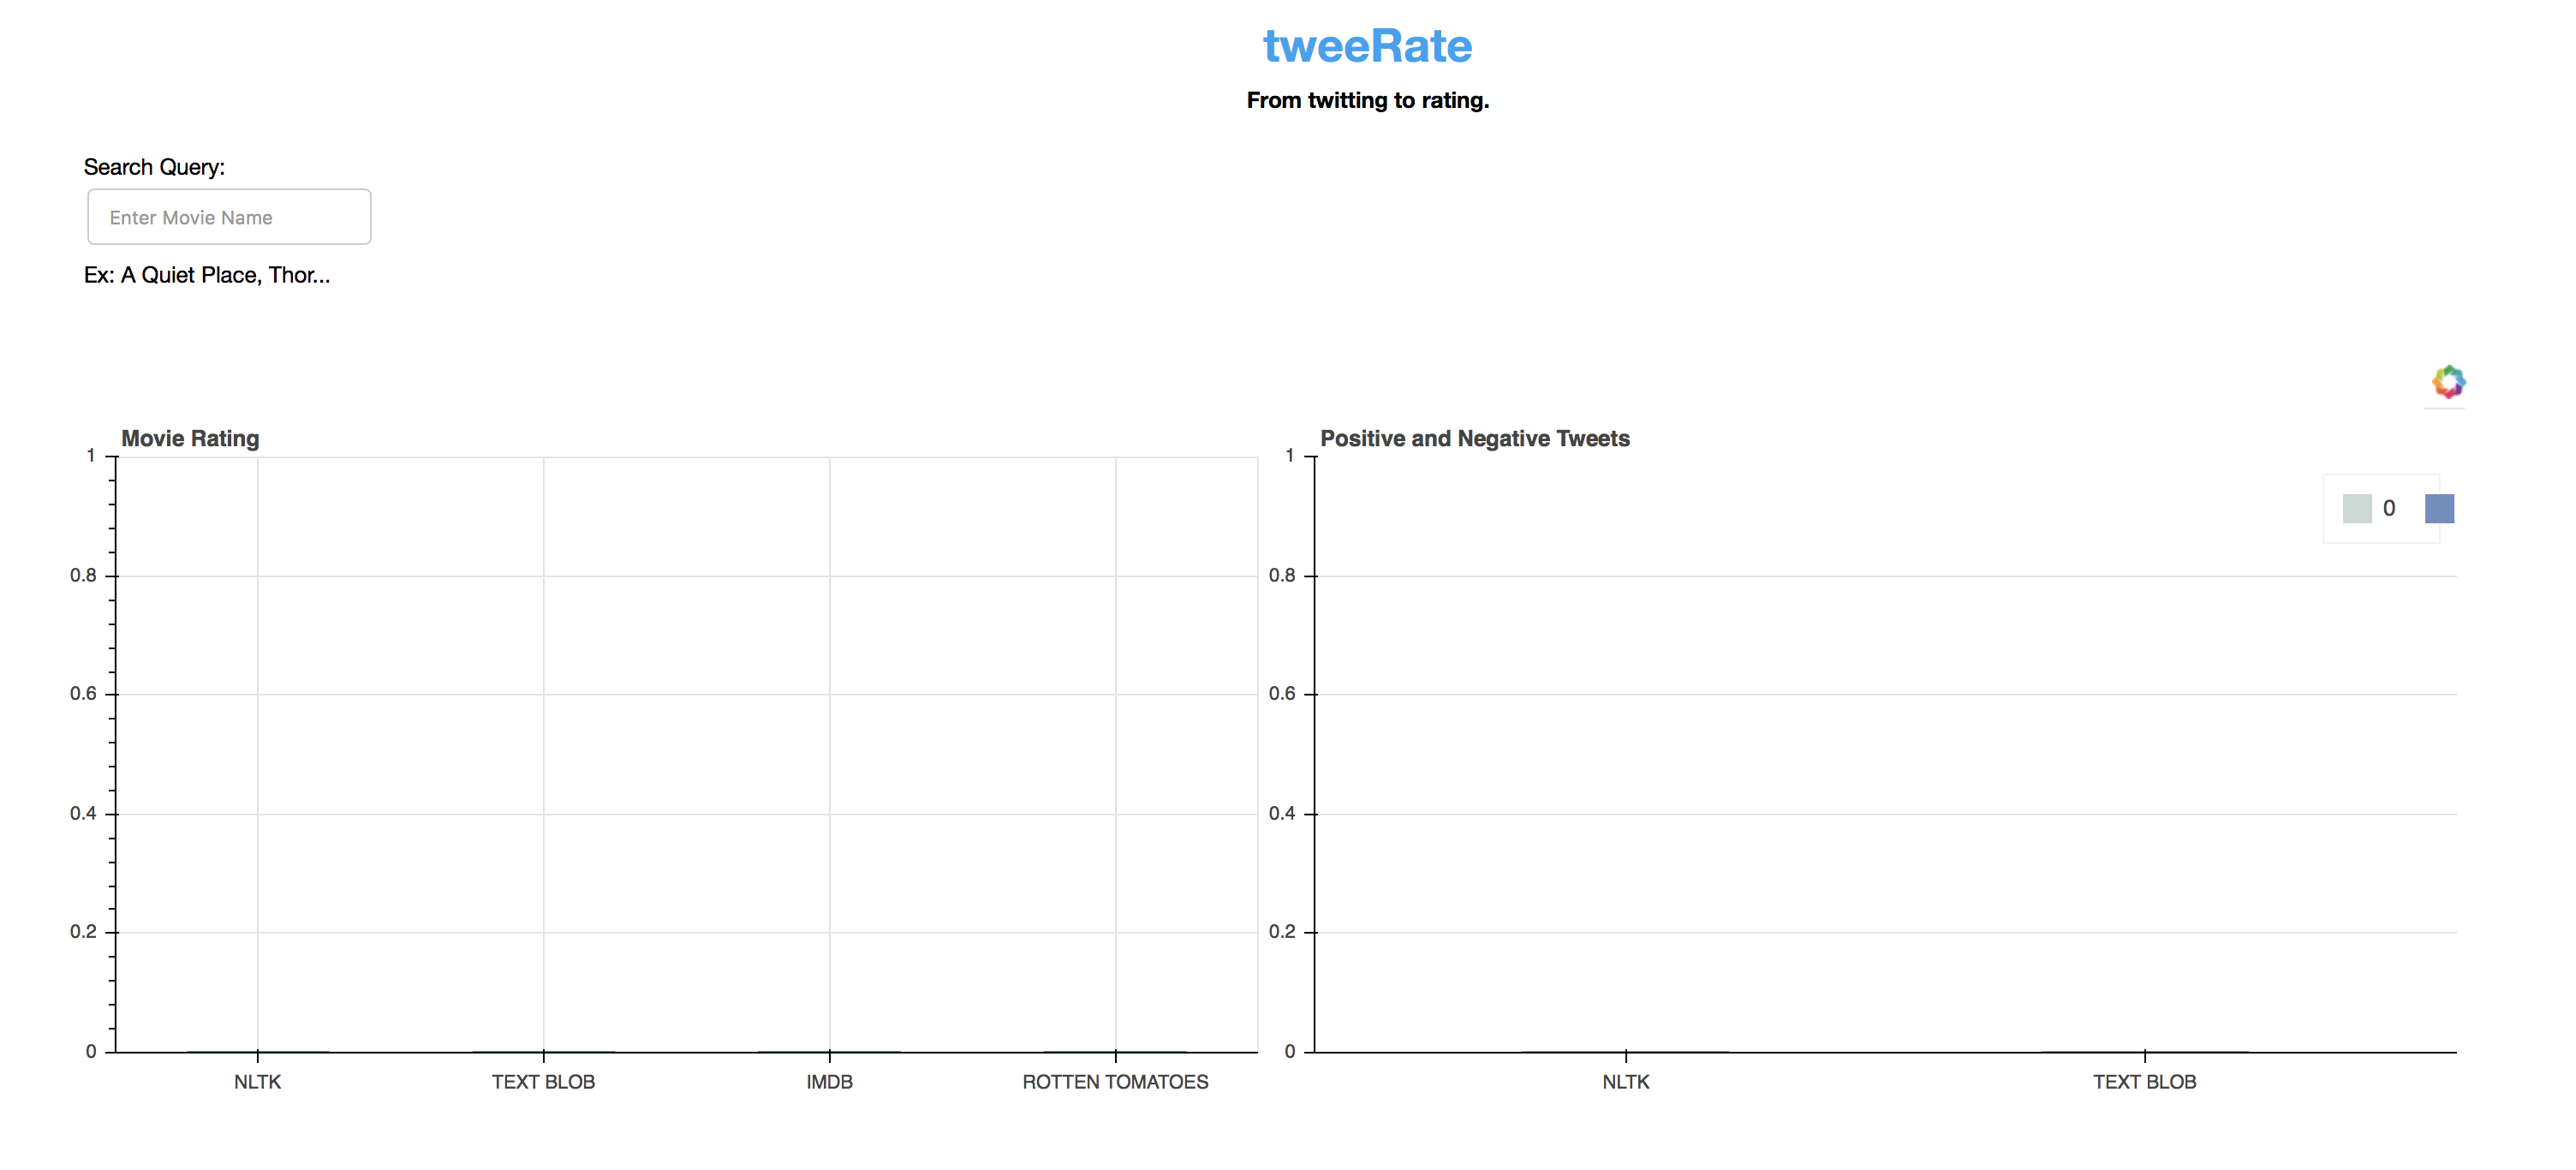
\includegraphics[width=1.0\textwidth]{Screen_Shot_2018-05-01_at_20_24_37.png}
\caption{\label{fig:blank}The Inputs are Blank}
\end{figure}\\ \\ \\
\begin{figure}
\centering
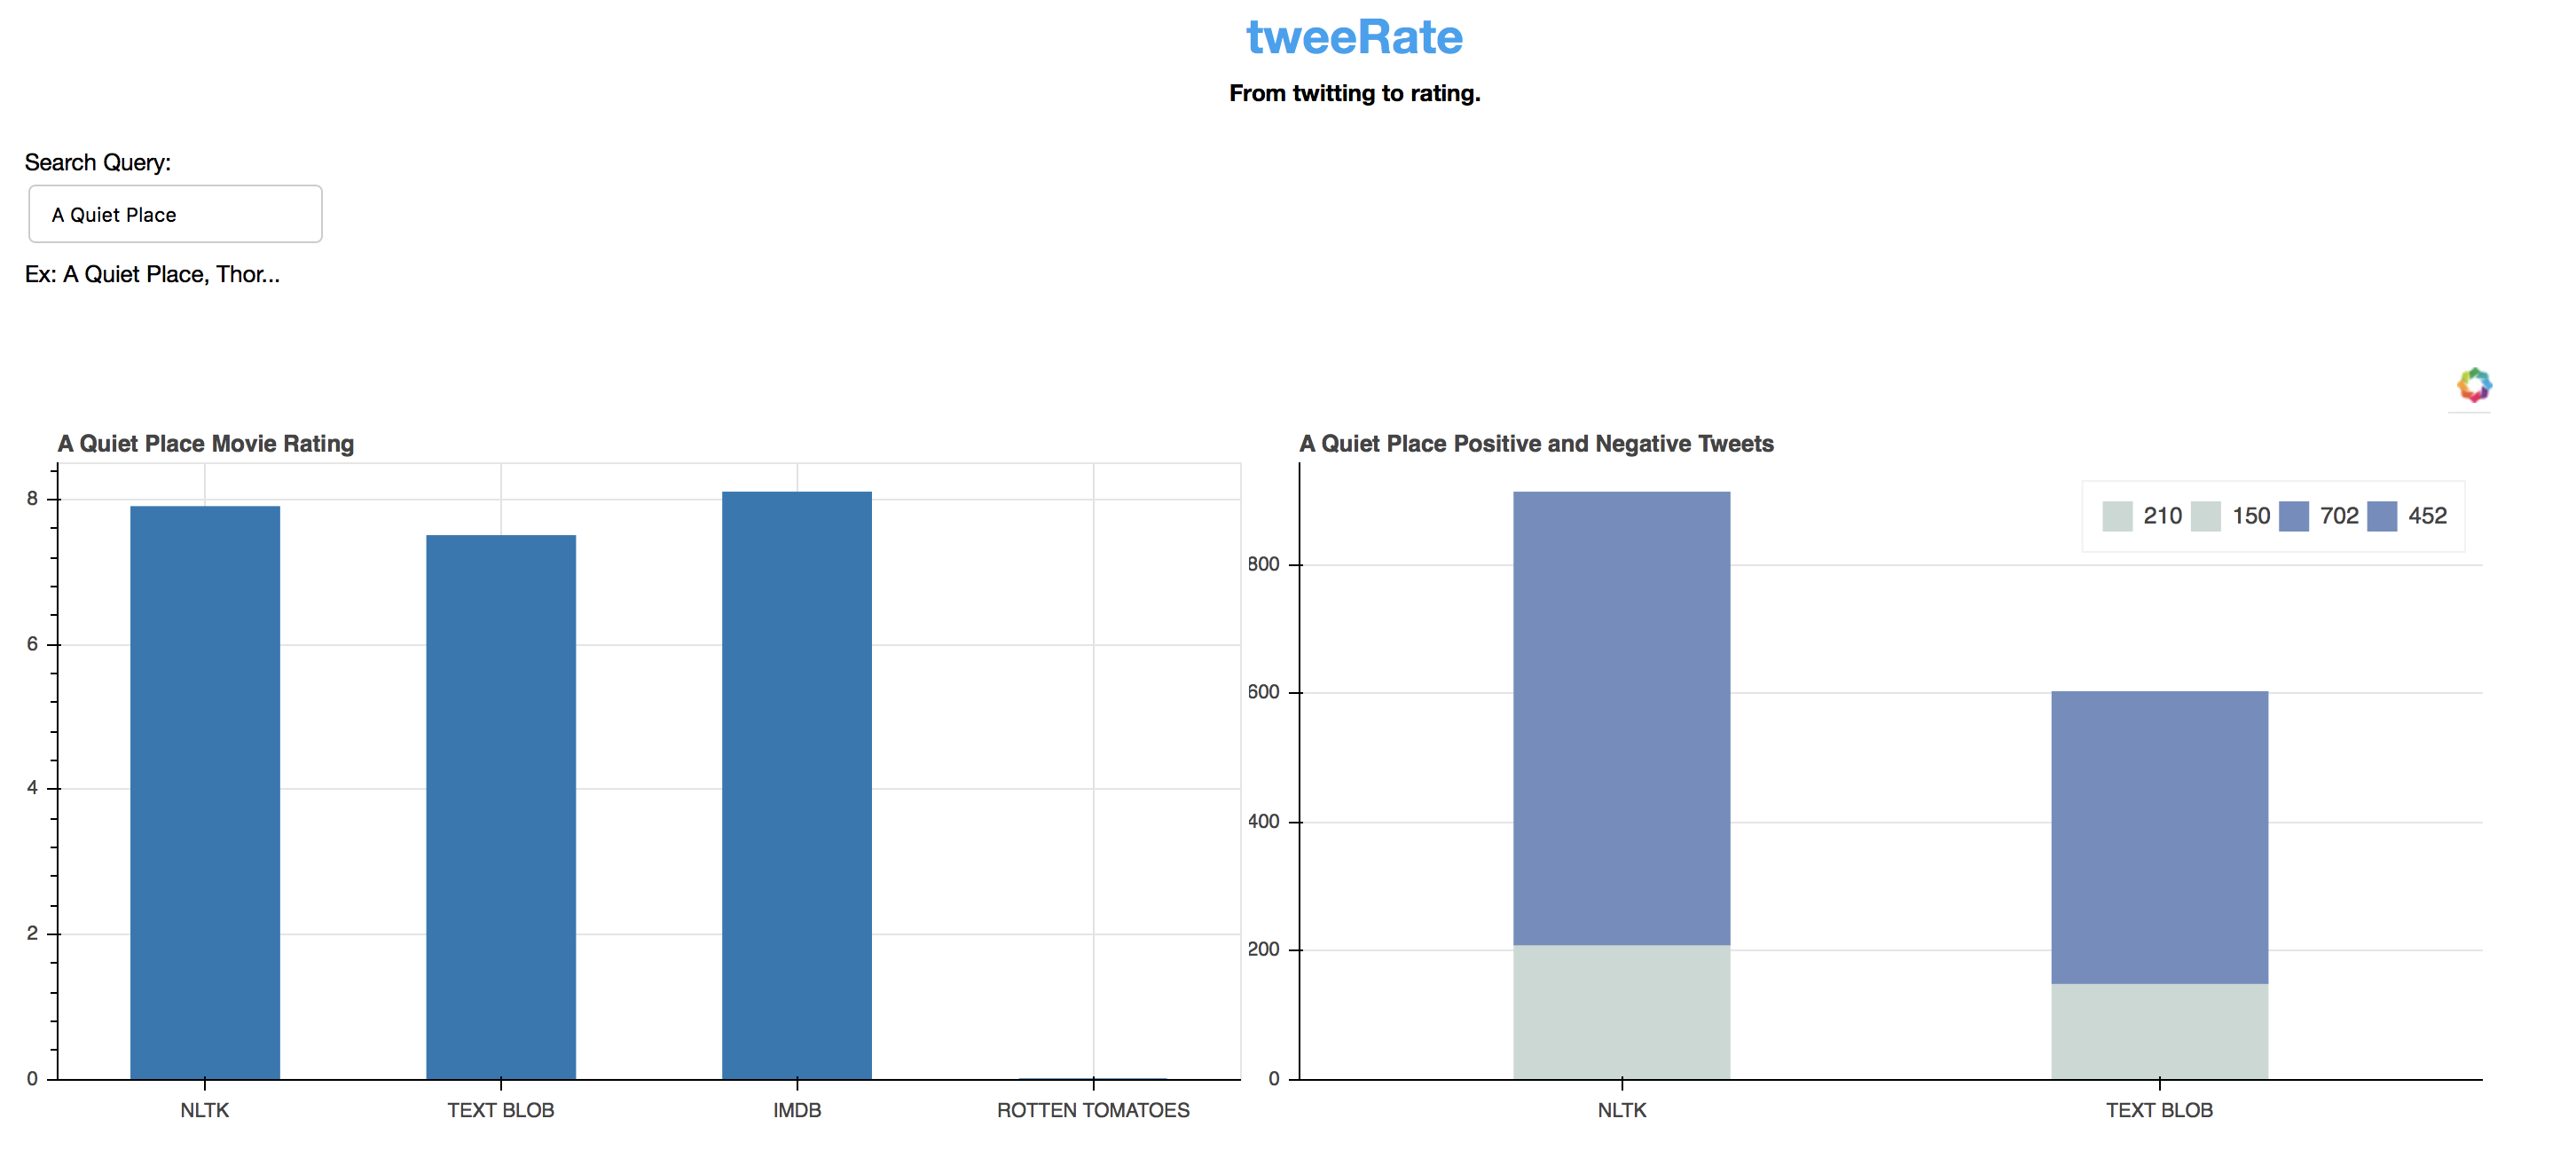
\includegraphics[width=1.0\textwidth]{Screen_Shot_2018-05-01_at_21_44_15.png}
\caption{\label{fig:result}The Above figure is having a input movie name as A Quite Place.}
\end{figure}
\begin{figure}
\centering
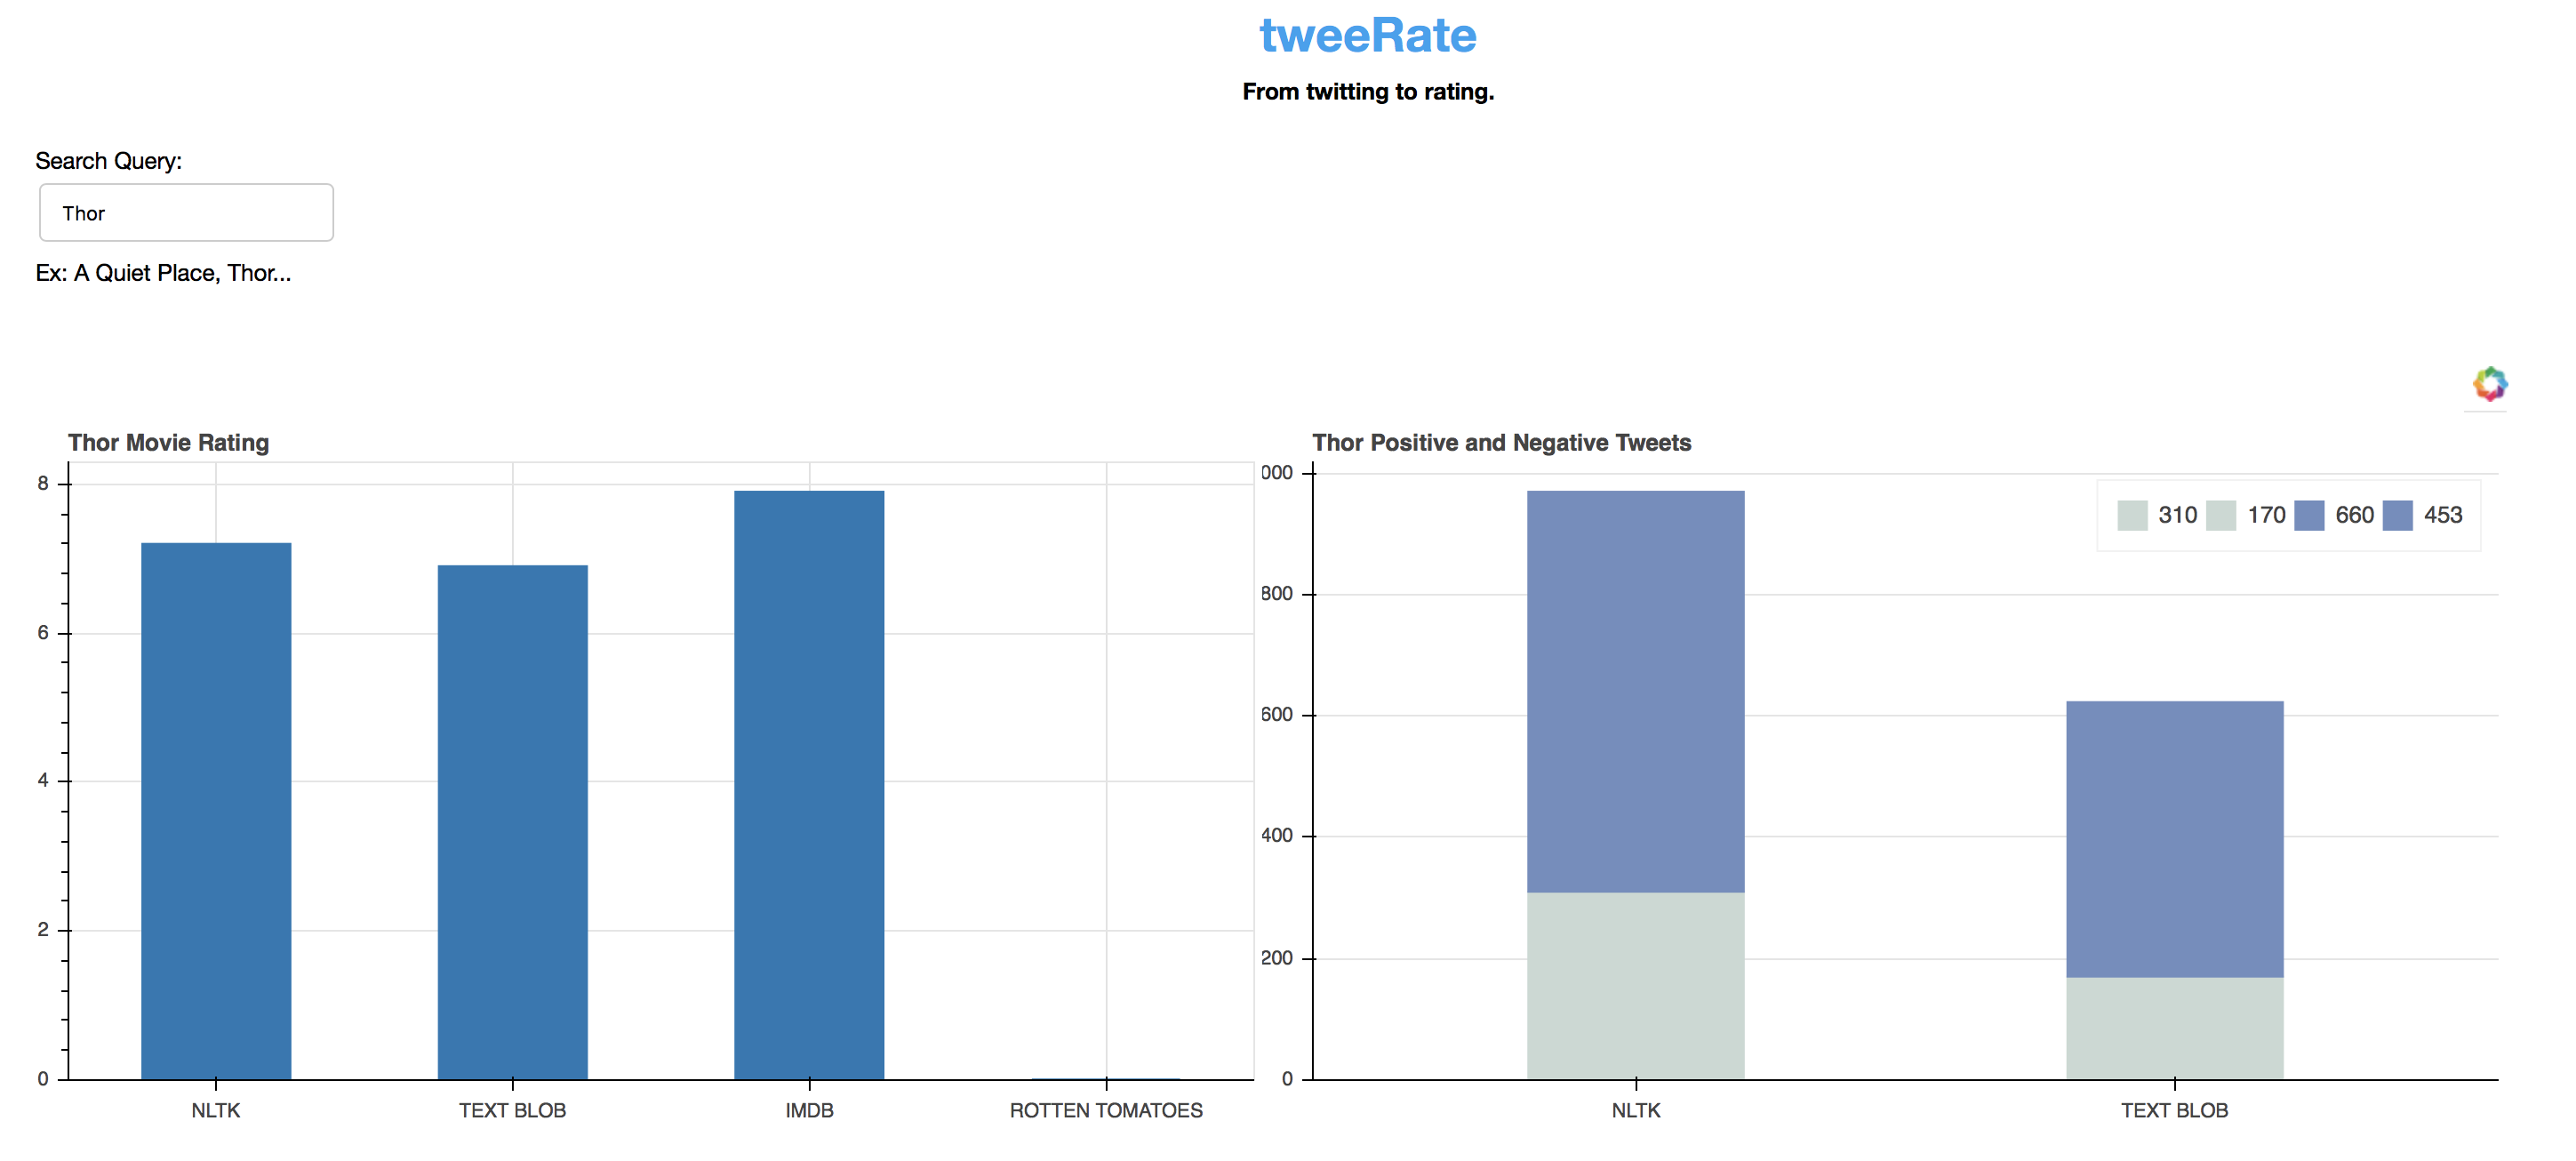
\includegraphics[width=1.0\textwidth]{Screen_Shot_2018-05-01_at_21_51_19.png}
\caption{\label{fig:result}The Above figure is having a input movie name as Thor}
\end{figure}

\section{CONCLUSION}
Twitter data effectively manages to capture the opinions and emotions of the crowd and Twitter APIs make it easy to gather this information and analyze it. This desktop application indeed manages to use this massive amount of data to provide a meaningful and useful result due to the speed limit introduced by Twitter, this is often presently an educational implementation of the thought to use twitter knowledge for rating a movie, in future if the limit on the information of twitter is removed then this application has excellent result and may be used for thus several merchandise review and its quality. If all the tweets containing the search string for a movie name will be captured and analyzed, a lot of precise conclusion will be drawn. The training data used by the classification algorithm are very limited for tweets per category. The results have been encouraging with the small set; We expect the result to be even more impressive with a larger selection of natural language processing in the training data. For some movies we predicted the exact rating but, in some cases, we are not getting exact result as we have some less data for that movie. As the application is used frequently, the dataset grows with it. This results in the rating of a movie always being up to date with public opinion. The best use case is to search for recent movies, simply because that is when the crowd seems to be tweeting most about the movies then more accurate rating will be predicted.
\section{Future Work}
In future enhancements, more categories can be introduced to classify tweets – extremely positive, mildly positive, extremely negative, mildly negative, neutral, and irrelevant. This can be used to improve the rating formula to make it more accurate. A weight can be associated with each category and then calculate the average.
More number of classes implies increase in number of attributes for the classifier to compare the input with. This should show some difference in the outcome of the classifier and hence difference in the rating shown by the application. We only consider the data from twitter but in future data from other social media like facebook, YouTube and other blogger comments is also taken into considerations for more accurate rating and with real opinions from all the social media into single place.
Along with that in future, we can compare multiple movies based on twitter sentiment analysis and plot comparison graph based on actor, director and music rating. Also we can predict which movie, actor, director, music will get the Oscar award based on people’s choice.
\begin{thebibliography}{9}
\bibitem{ref1} 
Aljaz Blatnik, Kaja Jarm, Marko Meza 
\textit{ Movie sentiment
analysis based on public tweets, Faculty of Electrical
Engineering, University of Ljubljana, Trzaska 25, 1000
Ljubljana, Slovenia}.
[\textit{On the electrodynamics of moving bodies}]. 
 81(4): 160–166, 2014 ORIGINAL
SCIENTIFIC PAPER.


\end{thebibliography}
\end{document}